\documentclass[a4paper]{article}
\usepackage{acronym}
\usepackage{amsmath}
\usepackage{forest}
\usepackage{tikz}
\usetikzlibrary{matrix,chains,positioning,decorations.pathreplacing,arrows}

\setlength{\parindent}{0em}
\setlength{\parskip}{1em}

\title{Mathematical background for CTRNN simulations}
\author{Øyvin Halfdan Thuv}

\begin{document}

\maketitle

\section{Equations for the Dynamics}
Equations are from an article\cite{beer-1995} of R. D. Beer, who did lots of interesting research into these networks.

\subsection{Neuron Activation Potential}
The activation potential (or firing-frequency) of each neuron is calculated by applying the sigmoid function in equation \ref{sigmoid-function} to the sum of the bias and the membrane potential.
\begin{equation}
  \label{sigmoid-function}
  \sigma(x) = \frac{1}{1 + e^{-x}}
\end{equation}

\subsection{Membrane Potentials}
Every neuron in a CTRNN maintains a state, the membrane potential. Neuron activation potentials at some specific network input will therefore vary depending on the current neuron states.

The change in membrane potential for each neuron is governed by the equation:
\begin{equation}
  \label{membrane-potential-equation}
  \dot{y}_i = \frac{1}{\tau_i}(-y_i + \sum_{j=1}^{N}w_{ji}\sigma(y_j + \theta_j) + I_i)
\end{equation}
\vspace{1em}
where\\
\begin{tabular}{ll}
  $\tau_i$: & time-constant of post-synaptic neuron\\
  $y_i$: & membrane potential of post-synaptic neuron\\
  $w_{ji}$: & weight of connection between pre-synaptic neuron $j$ and post-synaptic neuron\\
  $\sigma(x)$: & the sigmoid activation function in equation \ref{sigmoid-function}\\
  $y_j$: & membrane potential of pre-synaptic neuron $j$\\
  $\theta_j$: & bias (input sensivity) of pre-synaptic neuron $j$\\
  $I_i$: & any external input (such as a sensor reading) to post-synaptic node\\
\end{tabular}\par
\subsubsection{Procedure}
The clj-ctrnn library (at least currently) uses the \textit{forward Euler method} for approximating the solution to equation \ref{membrane-potential-equation} at a series of timesteps.

For each step in time, $t$, with $t<\tau_i$, clj-ctrnn will
\begin{enumerate}
\item Approximate the rate of membrane potential change, $\frac{\Delta y}{\Delta t}$, for all neurons
\item Synchronously update all membrane potentials $y_{i+1} = y_i + \frac{\Delta y}{\Delta t} \cdot t$
\item Commit the new network state
\end{enumerate}

\section{Specific Properties of the Model}
Some interesting properties of CTRNNs are bifurcative neurons and center-crossing networks.
\subsubsection{Bifurcative Neurons}
For neurons that connect to themselves with a synaptic connection $\geq4$, equation \ref{membrane-potential-equation} will have two solutions. In other words, the membrane potential may converge towards one of two possible steady-states.

Which one it converges to depends on previous membrane potential, so incjected current can trigger steady-state change. This can be a very useful property in pulse-circuits or sensor readings.

The following equations give the solutions to the left and right bifurcation points, respectively:
\begin{equation}
  lb(w_{ii},\theta) = 2 \cdot ln(\frac{\sqrt{w_{ii}} + \sqrt{w_{ii} - 4}}{2}) - \frac{w_{ii} + \sqrt{w_{ii} \cdot (w_{ii} - 4)}}{2} - \theta
\end{equation}
\begin{equation}
  rb(w_{ii},\theta) = -2 \cdot ln(\frac{\sqrt{w_{ii}} + \sqrt{w_{ii} - 4}}{2}) - \frac{w_{ii} - \sqrt{w_{ii} \cdot (w_{ii} - 4)}}{2} - \theta
\end{equation}

\subsubsection{Center-Crossing Networks}
Since the activation potential is calculated using the sigmoid function in equation \ref{sigmoid-function}, changes in input will yield most change in activation potential where existing input causes a neuron activation of $\approx 0.5$.

For a network with set weights, maximum inter-neuron sensivity can thus be achieved by setting the bias, $\theta$, for every neuron to some value that aligns their sum of bias and input to 0.
\begin{equation}
  \theta = \frac{-\Sigma_j^N{w_{ji}}}{2}
\end{equation}

\section{Calculations for the Tests}
For some of the tests, expected values are manually calculated.

\subsection{Single Neuron Network Test}
A network with a single neuron with one self-connection is one of the simplest tests. It has the following topology:\par
\begin{figure}[h]
  \centering
  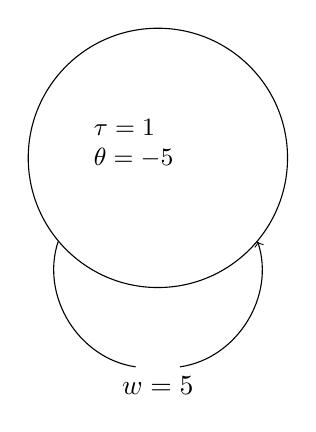
\begin{tikzpicture}[
      neuron/.style={
        draw,
        circle,
        inner sep=1em,
        font=\small
      }
    ]
    %% Neurons
    \node[neuron] (n-1) {\parbox[c][5em]{5em}{%
        $\tau = 1$\\
        $\theta = -5$\\
    }};
    %% Self 1
    \node[below=of n-1] (n-1-self) {$w=5$};
    \draw (n-1) edge[-, bend right=50] (n-1-self);
    \draw (n-1-self) edge[->, bend right=50] (n-1);
  \end{tikzpicture}\par
\end{figure}
Given equation \ref{membrane-potential-equation}, the membrane potential $y$ for each timestep $t$ of size $s$ can be written as:\par

\begin{equation}
  \footnotesize
  y(t,s) = y(t-s) + \dot{y}(t-s)
\end{equation}

Which can be expanded and simplified based on the neuron and network information above:
\begin{equation}
  \footnotesize
  \begin{aligned}
    \dot{y_i}(t) & = \frac{1}{\tau_i}(-y_i(t-1) + \sum_{j=1}^{N}w_{ji}\sigma(y_j(t-1) + \theta_j) + I_i)\\
    & \Downarrow\\
    \dot{y}(t) & = \frac{1}{1}(-y(t-1) + 5 \cdot \sigma(y(t - 1) - 5)\\
    & = -y(t-1) + 5 \cdot \sigma(y(t-1) - 5)\\
    & \Downarrow\\
    y(t,s) & = y(t-s) + s \cdot (-y(t-s) + 5 \cdot \sigma(y(t-1) - 5))
  \end{aligned}
\end{equation}
With timesteps = 0.01 the neuron membrane potentials can be approximated as follows for 5 steps to calculate reference values for testing:
\begin{equation}
  \footnotesize
  \begin{aligned}
    y(0.00) & = 0.000000\\
    y(0.01) & = 0.000000 + 0.01 \cdot (-0.000000 + 5 \cdot \frac{1}{1 + e^{-(0.000000 - 5)}}) = 0.000335\\
    y(0.02) & = 0.000335 + 0.01 \cdot (-0.000335 + 5 \cdot \frac{1}{1 + e^{-(0.000335 - 5)}}) = 0.000666\\
    y(0.03) & = 0.000666 + 0.01 \cdot (-0.000666 + 5 \cdot \frac{1}{1 + e^{-(0.000666 - 5)}}) = 0.000994\\
    y(0.04) & = 0.000994 + 0.01 \cdot (-0.000994 + 5 \cdot \frac{1}{1 + e^{-(0.000994 - 5)}}) = 0.001319\\
    y(0.05) & = 0.001319 + 0.01 \cdot (-0.001319 + 5 \cdot \frac{1}{1 + e^{-(0.001319 - 5)}}) = 0.001641\\
  \end{aligned}
\end{equation}

\subsection{Two Neuron Network}
A more complex two neuron center-crossing network with bifurcative neurons has the following topology:\par
\begin{figure}[h]
  \label{two-neuron-network}
  \centering
  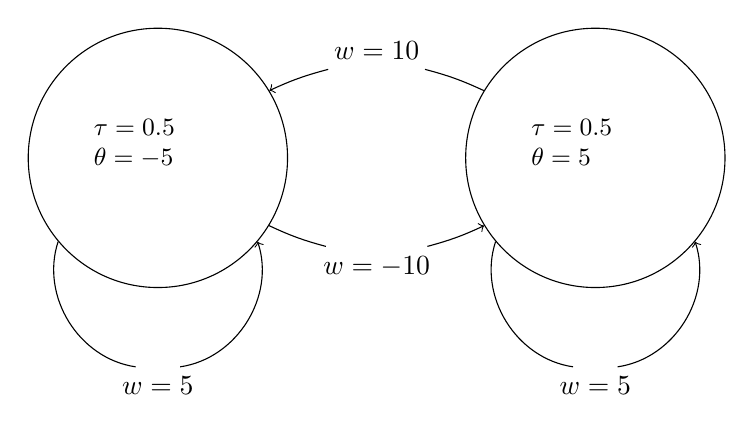
\begin{tikzpicture}[
      neuron/.style={
        draw,
        circle,
        inner sep=1em,
        font=\small
      }
    ]
    %% Neurons
    \node[neuron] (n-1) {\parbox[c][5em]{5em}{%
        $\tau = 0.5$\\
        $\theta = -5$\\
    }};
    \node[right=of n-1] (spacer) {};
    \node[right=of spacer,neuron] (n-2) {\parbox[c][5em]{5em}{%
        $\tau = 0.5$\\
        $\theta = 5$\\
    }};
    %% Synapses
    %% Self 1
    \node[below=of n-1] (n-1-self) {$w=5$};
    \draw (n-1) edge[-, bend right=50] (n-1-self);
    \draw (n-1-self) edge[->, bend right=50] (n-1);
    %% Self 2
    \node[below=of n-2] (n-2-self) {$w=5$};
    \draw (n-2) edge[-, bend right=50] (n-2-self);
    \draw (n-2-self) edge[->, bend right=50] (n-2);
    %% 1 -> 2
    \node[below=of spacer] (n-1-n-2) {$w=-10$};
    \draw (n-1) edge[-,bend right=5] (n-1-n-2);
    \draw (n-1-n-2) edge[->,bend right=5] (n-2);
    %% 2 -> 1
    \node[above=of spacer] (n-2-n-1) {$w=10$};
    \draw (n-2) edge[-,bend right=5] (n-2-n-1);
    \draw (n-2-n-1) edge[->,bend right=5] (n-1);
  \end{tikzpicture}
\end{figure}
The properties were chosen as follows:
\begin{enumerate}
\item The neurons are given  self-weights of 5 ($w_{ii}>4$).
\item The first neuron is given a bias of -5.
\item A synaptic connection from neuron two to neuron one is created, so that on average it will influence neuron one near the center of activations ($w=10$).
\item Neuron two is then set up with exactly opposite bias and opposite synaptic input from neuron one.
\end{enumerate}

\begin{figure}[h]
  \caption{Example plot of the activations of the neurons in \ref{two-neuron-network}.}
  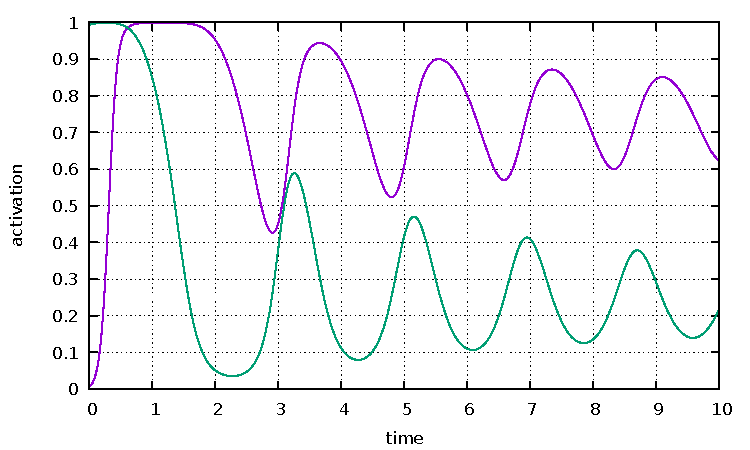
\includegraphics[width=0.9\textwidth]{plot.pdf}
\end{figure}

\begin{thebibliography}{9}

\bibitem{beer-1995}
  Randall D. Beer
  \textit{On the Dynamics of Small Continuous-Time Recurrent Neural Networks},
  Dept. of Computer Engineering and Science and Dept. of Biology
  Case Western Reserve University
  Cleveland, OH 44106
  1995

\end{thebibliography}

\end{document}
